\documentclass{TDP005mall}



\newcommand{\version}{Version 0.2}
\author{Niklas Åsberg, \url{nikas214@student.liu.se}}
\title{Designspecifikation}
\date{2023-11-24}
\rhead{Niklas Åsberg}
\graphicspath{{./}}

\begin{document}
\projectpage
\section{Revisionshistorik}
\begin{table}[!h]
\begin{tabularx}{\linewidth}{|l|X|l|}
\hline
Ver. & Revisionsbeskrivning & Datum \\\hline
0.1 & Utkast & 2023-11-21 \\\hline
0.2 & Ändrad design efter feedback på kravspecen & 2023-11-24 \\\hline
\end{tabularx}
\end{table}

\tableofcontents
\newpage

\section{Introduction}
I det här dokumentet så beskrivs designen av mitt spel. Jag kommer att gå igenom två av mina klasser i detalj och sen visa UML-diagrammet över alla mina klasser. \\
Avslutningsvis diskuterar jag mina designval.

\section{Detaljbeskrivning}
Två av mina klasser kan vara extra intressanta att analysera: Playerklassen och Squareklassen.

\subsection{Playerklassen}
Playerklassen ska representera spelaren. Klassen implementerar Characterklassen som i sin tur ärver från GameObjectklassen. \\
Playerklassen interagerar direkt med en annan klass, Squareklassen. 
\subsubsection{Attribut}
Dessa attribut är specificerade i Characterklassen som är en interface som i sin tur ärver av GameObjectklassen.
\begin{itemize}
  \item int: health - antalet liv spelaren har.
  \item float: speed - hur snabbt spelaren kan röra sig.
  \item int: damage - hur mycket skada spelaren gör när den attackerar.
  \item sf::Time: timeSinceDamaged - tiden sen spelaren sist blev skadad.
  \item sf::vector2f: location - positionen som spelaren har just nu.
  \item string: sprite - filvägen till spelarens bild.
  \item bool: collidable - bool som visar om det går att kollidera med spelaren
  \item int: size - storleken på spelaren.
\end{itemize}
\subsubsection{Metoder}
Metoden attack() är den enda metoden som är unik för Playerklassen, de andra metoderna är specificerade i interfacet.
\begin{itemize}
  \item onCollision() - vad som händer om en spelare kolliderar med någonting annat.
  \item move() - metod för att flytta spelaren.
  \item attack() - metod för att attackera.
\end{itemize}

\newpage

\subsection{Mapklassen}
Mapklassen representerar spelplanen. Spelplanen innehåller alla objekt som implementerar GameObjectklassen. \\
Mapklassen interagerar med GameObjectklassen för att kunna avgöra om en kollision har inträffat. \\
\subsubsection{Attribut}
\begin{itemize}
  \item GameObject[]: gameObjects - en lista av referenser till alla instanser av GameObjectklassen.
\end{itemize}
\subsubsection{Metoder}
\begin{itemize}
  \item allowedPosition() - anropas av ett objekt som vill flytta för att se om en kollision kommer ske.
\end{itemize}

\section{UML-diagram}
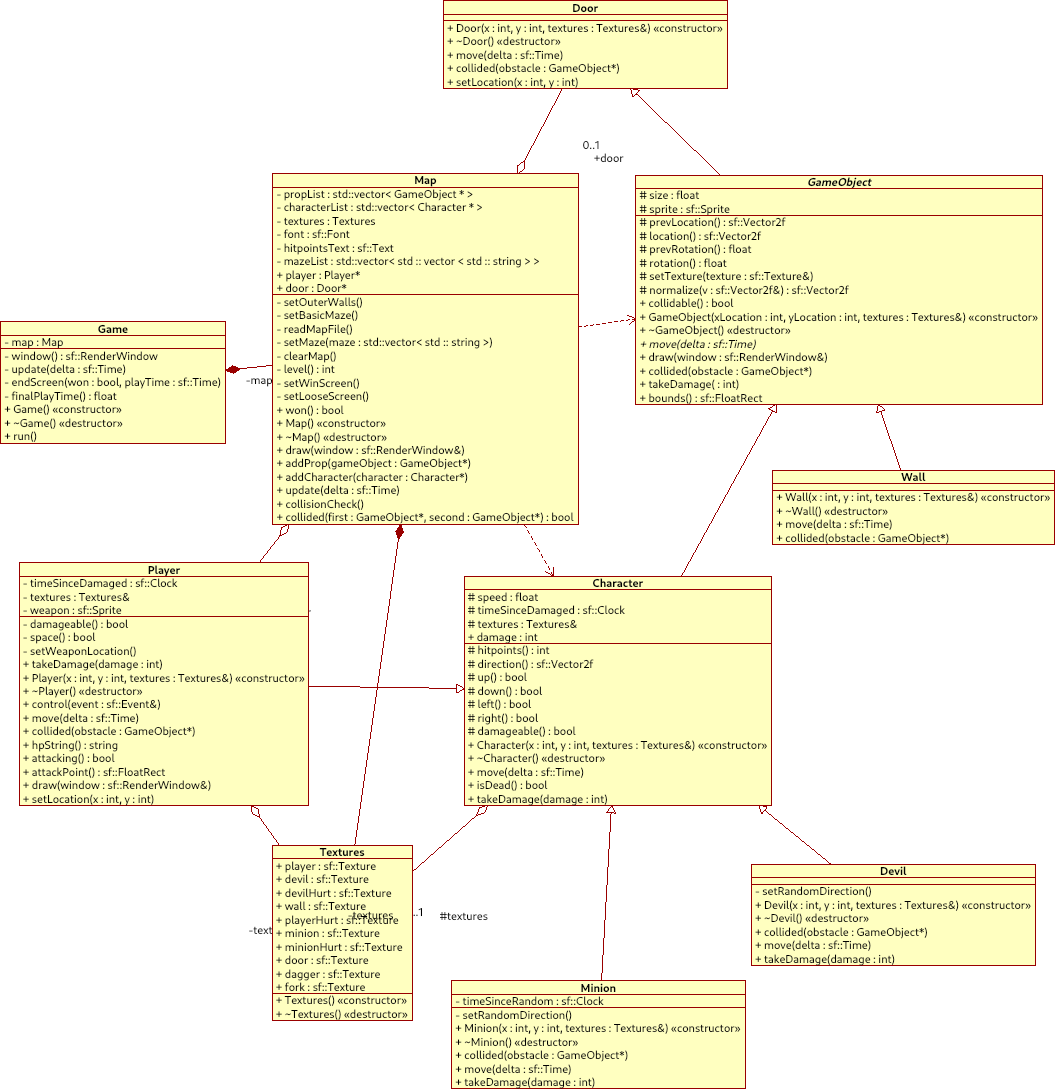
\includegraphics[scale=0.52]{uml-diagram}

\newpage
\section{Diskution}
I mitt spel så utgår allt från en instans av Gameklassen, Gameklassen innehåller en instans av Mapklassen. Gameklassen har även ansvaret att byta instansen \\
av map när en ny bana påbörjas, Gameklassen sköter inladdningen av ban-filen och skapar Map-instansen från den. 
Map-instansen innehåller alla GameObject-instanser, och har koll på om objekt har kolliderat.
Jag valde den här typen av design då det blir väldigt lätt att lägga till och ändra hur spelet ska se ut. \\
Om man till exempel vill lägga till andra hinder eller karaktärer så behöver vi inte ändra i de allra flesta klasser.
Kollisionshanteringen sker mellan spelobjekt så om vi skulle vilja ändra vad som händer vid kollision så ändrar vi bara i det spelobjektets klass.
Tanken är att minska coupling och ha hög cohesion.

\section{Externa filformat}
Om vi bortser från png-filerna som bara är där för esteriska skäl så är det enda externa filformatet det för banorna.
Mitt spel använder sig av en enkel fil där specifikationen för banan är skiven i text, ett tecken för varje ruta med olika tecken för varje objekt.

\end{document}
